%%%% ijcai19-multiauthor.tex

\typeout{IJCAI-19 Multiple authors example}

% These are the instructions for authors for IJCAI-19.

\documentclass{article}
\pdfpagewidth=8.5in
\pdfpageheight=11in
% The file ijcai19.sty is NOT the same than previous years'
\usepackage{ijcai19}

% Use the postscript times font!
\usepackage{times}
\usepackage{soul}
\usepackage{url}
\usepackage{graphicx}
\usepackage[hidelinks]{hyperref}
\usepackage[utf8]{inputenc}
\usepackage[small]{caption}
\usepackage{graphicx}
\usepackage{amsmath}
\usepackage{booktabs}
% installez ce package -> sudo apt-get install texlive-science
\usepackage[ruled,vlined]{algorithm2e}
\urlstyle{same}
\usepackage{biblatex}
\addbibresource{ijcai19.bib}

% the following package is optional:
%\usepackage{latexsym} 

% Following comment is from ijcai97-submit.tex:
% The preparation of these files was supported by Schlumberger Palo Alto
% Research, AT\&T Bell Laboratories, and Morgan Kaufmann Publishers.
% Shirley Jowell, of Morgan Kaufmann Publishers, and Peter F.
% Patel-Schneider, of AT\&T Bell Laboratories collaborated on their
% preparation.

% These instructions can be modified and used in other conferences as long
% as credit to the authors and supporting agencies is retained, this notice
% is not changed, and further modification or reuse is not restricted.
% Neither Shirley Jowell nor Peter F. Patel-Schneider can be listed as
% contacts for providing assistance without their prior permission.

% To use for other conferences, change references to files and the
% conference appropriate and use other authors, contacts, publishers, and
% organizations.
% Also change the deadline and address for returning papers and the length and
% page charge instructions.
% Put where the files are available in the appropriate places.

\title{Entrainement d'un agent virtuel par Q-learning pour le jeu Snake}

\author{
Samuel Ferron\and
Jean-Frédéric Fontaine\and
Noboru Yoshida
\affiliations
Department de génie logiciel, Polytechnique Montréal, Canada\\
\emails
\{samuel.ferron, jean-frederic.fontaine, noboru.yoshida\}@polymtl.ca
}

\begin{document}

\maketitle

\begin{abstract}
Le présent rapport a été réalisé dans le cadre du cours INF8225 - Intelligence artificielle : techniques probabilistes et d’apprentissage. Le but de ce rapport est d'expliciter en détail le processus par lequel nous avons implémenté un algorithme présenté dans un papier scientifique ayant pour sujet un thème présenté en classe. Nous avons donc implémenté le jeu de Snake et nous avons entrainé un agent intelligent avec la technique de Q-learning. Nous avons obtenu les résultats similaires au papier d'origine. 
\end{abstract}

\section{Introduction}

Depuis 1997, lorsque Deep Blue a battu Garry Kasparov, ex-champion du monde d’échecs, de nombreux chercheurs se sont lancés dans la recherche d’algorithmes afin de battre les champions humain dans les jeux les plus connus. Aujourd’hui, il existe des réseaux neuronaux qui performent mieux que l'homme aux échecs, mais aussi à Go et au Shogi. En 2019, un projet nommé AlphaStar a réussi à battre des joueurs humains dans StarCraft II; un jeu vidéo stratégique qui se joue en ligne.\linebreak

Nous nous sommes intéressés au fonctionnement de ces réseaux neuronaux et nous avons donc décidé d’en implémenter un nous-mêmes, avec le fameux jeu de Snake.\linebreak

Ce papier présente une revue de la littérature, une description brève du jeu Snake qui consiste notre environnement d'application, une explication théorique de l'algorithme principal utilisé, soit celui du Q-Learning, un compte-rendu de notre expérience avec son implémentation, les résultats obtenus et finalement un retour sur ce dernier.

\section{Revue de la littérature}
 
Le type d'apprentissage par renforcement moderne a été introduit dans le monde de l'intelligence artificielle dans les années 1960 lorsque Michie a implémenté une machine qui apprend à jouer un jeu de tic-tac-toe (\cite{10.1093/comjnl/6.3.232}). La machine a été initialement construite avec des boîtes d'allumettes et un ordinateur Pegasus 2 roulait un programme qui exécutait une séquence d'actions basée sur la méthode essai-erreur. À chaque itération, la machine garderait en mémoire le résultat (victoire, égalité ou défaite) et la séquence d'actions exécutées. Elle peut ainsi apprendre, suite à de nombreux essais, les séries de séquences à éviter pour ne pas perdre et les actions qui lui permettraient de décrocher une victoire.
\linebreak

La méthode d'essai-erreur utilisée lors de cette expérience a été améliorée au fil des années et de nouvelles expériences ont été réalisées sur d'autres jeux comme le Backgammon. Tesauro (\cite{tesauro_sejnowski_1989}) a effectivement implémenté réseau neuronal qui tente de reconnaitre des règles à partir d'une suite de valeurs de sorties. Ainsi, il réussit à modéliser un réseau pouvant choisir une action qui est avantageuse pour le joueur virtuel plutôt que d'en générer une aléatoirement et vérifier si c'est la bonne option.
\linebreak

Plus tard, le monde de l'apprentissage profond connait un changement drastique avec des chercheurs l'appliquant dans une multitude de domaines différents. En effet, des spécialistes de la reconnaissance de la parole (\cite{dahl_yu_deng_acero_2012}) tentent d'implémenter un modèle se servant d'un réseau de neurones à  profond avec un  automate de Markov à états cachés. Aussi,  des chercheurs dans le domaine de la vision artificielle (\cite{krizhevsky_sutskever_hinton_2017}) ont également commencé à utiliser des modèles d'apprentissage profond en particulié des réseaux neuronaux convolutifs afin d'augmenter l'efficacité et la précision de leur modèle. Google utilise de nos jours un modèle d'apprentissage machine pour leurs services de traduction automatique (\cite{DBLP:journals/corr/WuSCLNMKCGMKSJL16}). En utilisant deux types de réseaux de neurones, un pour traiter les données entrantes et un autre pour générer le texte qui a été traduit, il peut améliorer la qualité de leur service en continuant à l'entrainer. Ces avancements technologiques ont permis aux chercheurs en apprentissage par renforcement d'essayer de nouvelles méthodes qui leur permettraient potentiellement d'améliorer leurs modèles.
\linebreak

Peu importe la complexité du jeu, le concept d'apprentissage par renforcement demeure relativement semblable. En effet, il faut d'abord créer un environnement à partir duquel on peut retirer des informations, c'est-à-dire un état
qu'on peut présenter à un agent afin qu'il puisse se représenter son environnement. Même dans un jeu de stratégie très complexe comme celui de StarCraft II \cite{DBLP:journals/corr/abs-1708-04782}, les chercheurs ont réussi à concevoir un environnement d'apprentissage par renforcement, qui a d'ailleurs été utilisé pour implémenter l'algorithme de AlphaStar. Pour ce faire, chaque détails du jeu ont été analysés de manière minutieuse et a ensuite été transformé en variables et matrices. Ces données représentant le grand nombre de ressources et d'influence, ainsi que les centaines de pièces que le joueur doit bouger sont ensuite utilisées pour calculer les actions que le modèle doit exécuter afin de maximiser sa récompense. Le défi en apprentissage par renfocement est donc de générer une représentation de l'état de l'environnement et de créer une politique de renforcement cohérente avec le but du jeux. \linebreak

Dans ce travail, nous avons émulé l'expérience réalisée par Mnih et al. \cite{DBLP:journals/corr/MnihKSGAWR13} qui consiste à créer un modèle ayant les capacités de jouer à des jeux d'Atari 2600. Dans leur papier, ils expliquent chaque étape de leur processus, en particulier l'algorithme Q-learning et l'architecture du réseaux qu'ils on mis en place. Le Q-learning est une méthode qui se base sur une approche de programmation dynamique incrémentale utilisant une méthode de Monte-Carlo afin d'estimer une valeur de sortie optimale. Elle a été améliorée par Watkins en 1989 (\cite{article}) et est encore appliquée dans des expériences de nos jours. 

\section{Explication du jeu Snake }
Le jeu de Snake consiste en un environnement fermé 2D dans lequel une représentation simplifiée (en pixel) d'un serpent doit atteindre un point, qui consiste à de la nourriture, afin d'accumuler des points. Lorsque le point est atteint, le serpent augmente de taille. Si le serpent entre en contact avec lui-même ou encore avec une paroi de l'environnement; la partie est terminée. Ainsi, le jeu devient de plus en plus difficile étant donné que la longueur du serpent augmente et la capacité de celui-ci à faire certains déplacements diminue. Certaines versions du jeu accélèrent aussi la vitesse de déplacement du serpent en plus de sa taille. Dans notre implémentation, nous n'avons pas ajouté cette fonctionnalité, car la vitesse à laquelle l'agent prend une décision nous importe peu (l'horloge d'un processeur est beaucoup plus rapide que la vitesse maximale à laquelle un humain peut jouer), c'est plutôt la qualité de la décision qui nous importe. La figure 1 montre l'interface de notre jeu de Snake. À gauche de la figure, on témoigne d'un Snake en début de partie et à droite après quelques minutes de jeu. 
\begin{figure}[ht]
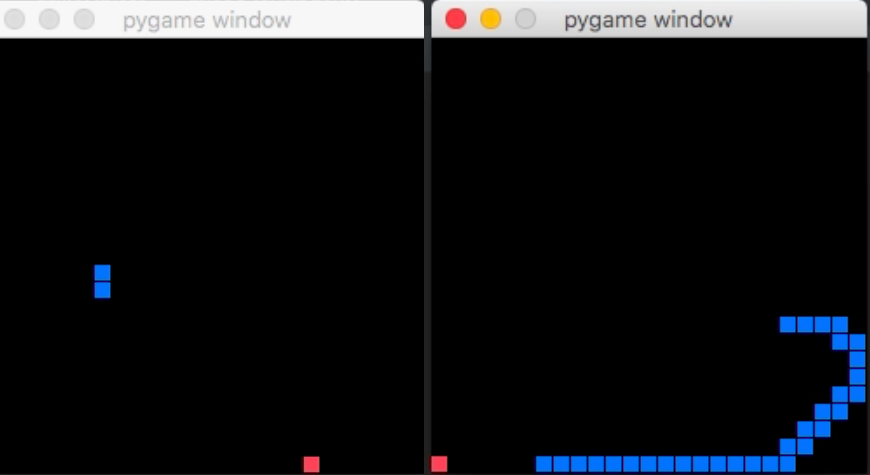
\includegraphics[width=\linewidth]{snake.png}
\caption{Snake qui augmente sa taille en atteignant la cible.}
\label{fig:Snake}
\end{figure}

\section{Q-Learning : Explication théorique  }
Généralement, les algorithmes d’apprentissages machines dépendent d’une grande quantité de données qui ont été étiquetées à la main afin de pouvoir faire des prédictions de qualité. Cependant, dans le contexte de l'apprentissage par renforcement, l’idée est plutôt de permettre à un l’algorithme, c’est-à-dire un agent, d’apprendre par lui-même les règles qui définissent le succès ou l’échec d’une tâche quelconque.\linebreak

Afin de nous familiariser avec l'algorithme de Q-learning nous avons entrainé un agent à jouer au jeu de Snake selon une politique de renforcement relativement simple. Pour ce faire, nous avons émulé l'expérience réalisée par Mnih et al. \cite{DBLP:journals/corr/MnihKSGAWR13}. Dans cette procédure, les chercheurs ont entrainé un agent virtuel à jouer à plusieurs jeux Atari. L'agent consiste en un réseau de neurones à convolution qui reçoit comme entrée la représentation visuelle du jeu, c'est-à-dire une image 210 X 160 pixels RGB. L'agent est ensuite entrainé par l'algorithme de Q-Learning selon une procédure de renforcement ( i.e récompense). En s'inspirant de cette approche et du blog de Comi \cite{comi_2020}, nous avons mis en place une procédure similaire avec la seule différence que nous fournissons à l'agent une représentation simplifiée de l'état de la partie et non une image. Plus précisément, considérons un agent virtuel qui intéragit avec l'environnement $\xi$ (i.e. le Snake), dans notre cas, un environnement 2D fermé, au Snake et à la nourriture que celui-ci doit atteindre afin de recevoir une récompense. À chaque époque temporelle, c'est-à-dire, à chaque nouveau déplacement du Snake, l'agent doit choisir une action $a_t$ au temps $t-1$ parmi l'ensemble d'actions légales $\Delta  = \{1, ..., K\}$. Une fois l'action choisie, celle-ci est exécutée. Cette action a pour effet de modifier l'état interne de la partie. Afin d'éxécuter une nouvelle action au temps $t$, nous fournissons à l'agent le nouvel état ainsi qu'une récompense si son action au temps $t-1$ le mérite. Dans notre approche, nous fournissons à l'agent une représentation simplifiée de la partie basée sur l'imminence d'un danger et la direction de la nourriture du Snake. Nous considérons donc pour le temps $t-1$ un vecteur qui décrit l'état de la partie et l'action qui a été prise pour cet état $s_t = x_{1}, a_{1}$. La prochaine action de l'agent pour le temps $t$ sera basée sur le vecteur $s_t$. Le but de l'agent est donc de choisir une nouvelle action afin de maximiser une récompense future (ou minimiser les renforcements négatifs). Afin d'entrainer l'agent, nous définissons la fonction d'action optimale $Q^*(s,a)$ qui consiste au renforcement maximal attendu en suivant n'importe qu'elle stratégie après avoir vue un état $s$ et avoir pris une action $a$, c'est-à-dire que $Q^*(s,a)= max_\pi 	\mathrm{E} \{R_t | s_t = s, a_{t} = a, \pi\}$ où $\pi$ est une politique qui associe un état de la partie à une action.  La fonction d'action optimale obéit une identité importante appelée équation de \textit{Bellman}. L'idée derrière cette équation est la suivante: si la valeur optimale de $Q^*(s',a')$ à l'état $s'$ était connue pour toute les actions possibles $a'$, alors la stratégie optimale est de choisir l'action $a'$ qui maximise le renforcement attendu pour $r + \gamma Q^*(s',a')$. Dans le contexte de l'apprentissage par renforcement, nous pouvons chercher une solution qui approxime $Q^*$ en incorporant dans un réseau de neurones la fonction 

$$NewQ(s,a) = Q(s,a)  + \alpha [\ R(s,a) + \gamma maxQ{'} (s{'},a{'}) - Q(s,a) ]\ $$

où $NewQ(s,a) $ correspond à la nouvelle récompense attendue au temps $t$, $Q(s,a)$ à la récompense approximée au temps $t-1$ correspondant à l'action prise au temps $t-1$, $\alpha$ au taux d'apprentissage, $R(s,a)$ à la récompense donnée pour cette action, $\gamma$ au "Discount rate" (constante souvent initialisée à .99) et $maxQ{'} (s{'},a{'})$ à la valeur maximale de la récompense attendue pour toutes les actions possibles (qui correspond à la sortie du réseau de neurones). Ainsi, nous appliquons cette formule de façon itérative et nous optimisons la fonction de perte de type MSE (Mean Squared Error)  $L( \theta_{i}) = [\ y_{i} - Q(s,a; \theta_{i})^{2} ]\ $. Autrement dit, l'agent estime la meilleure action à prendre selon la récompense attendue. À la prochaine iétration, on estime à nouveau la même action selon le même état en sachant la récompense que cette action a réeellement donnée. On calcule la différence entre l'estimation et la récompense réellement atteinte (la fonction de perte) puis on ajuste les poids à l'aide de la descente du gradient. De plus, pour toutes les parties, nous enregistrons en mémoire chaque action prise par l'agent ainsi que les états et les récompenses obtenues. À la fin de chaque partie, nous prenons un échantillon qui représente autant les actions qui ont provoqué un renforcement positif que les actions qui ont provoqué un renforcement négatif. Ainsi, nous procédons à une deuxième phase d'apprentissage entre les parties en fonctions de ces échantillons. Ceci permet à l'agent d'être proportionnellement entrainé sur des situations qui pourraient arriver moins souvent (e.g trouver la nourriture). 

Il suffit ensuite de remplacer la nouvelle valeur de récompense attendue au temps $t$.

\section{Explication de notre implémentation}

L’implémentation proposée peut se diviser en trois parties distinctes: le jeu, l’agent et le contrôleur.

Premièrement le jeu. L’objectif du projet est d’entrainer un DQN sur le jeu classique Snake, il nous faut donc une forme du jeu pour laquelle nous aurons accès à son état et à son contrôle. Nous avons choisi de recréer le jeu en Python à l’aide de la librairie PyGame. Tout d'abord, il faut définir l’état qui sera utilisé pour entrainer l’agent. L’état représente l’environnement dans lequel le serpent se retrouve à un temps donné. Il représente aussi l’entrée de notre modèle. Dans notre cas, l’état aura la forme d’un vecteur avec 11 valeurs booléennes qui indiquent les situations suivantes:

\begin{itemize}
	\item Si la nourriture est à gauche, en face, à droite ou en arrière du serpent.
	\item S'il y a un danger imminent à gauche, en face ou à droite du serpent.
	\item La direction du serpent (gauche, haut, droite ou bas).
\end{itemize}

Les actions possibles pour l'agent sont: aller à gauche, continuer dans la même direction ou aller à droite.

L’agent est quant à lui l’entité qui contient le modèle d’apprentissage et qui doit effectuer les meilleures actions à prendre selon un état donné. Nous utilisons un réseau de neurones profond. Il contient trois couches cachées, contenant 120 neurones munis de fonctions d'activations de type ReLU, et d’une couche finale de type Softmax à trois sorties, une pour chaque action. L’agent est entrainé à chaque pas que le serpent fait et conserve une mémoire qui lui permet un entrainement en lot entre les parties. L’entrainement d’un pas considère l’état original du pas, l’action prise, l’état actuel ainsi que la récompense obtenue suite à l’action. Le système de récompense est simple; si le serpent perd, la récompense est mise à -10. Si le serpent mange, la récompense est mise à 10.

Troisièmement, le contrôleur est ce qui orchestre l'interaction entre le jeu et l’agent. Ce code implémente l’algorithme Deep Q-Learning. Nous utilisons une variable, epsilon, qui permet d’effectuer une action aléatoire selon une probabilité. Cette variable dégrade entre chaque partie et promue l’exploration dans les premières époques de l’entrainement. Le programme se déroule comme suit:

\begin{algorithm}
\caption{Séquence d'entrainement de l'agent}
\KwResult{Un agent intelligent entrainé}
initialisation\;
\For{i in epochs}{
	initialisation du jeu\;
	entrainer l'agent avec sa mémoire\;
	\While{not done}{
		Prendre l'état actuel\;
		Prédire les récompenses associées à chaque action possible par le modèle\;
		Effectuer l'action qui favorise la meilleure récompense\;
		Prendre le nouvel état\;
		Calculer la récompense selon le nouvel état\;
		Comparer la récompense obtenue avec celle prédite (fonction de perte)\;
		Entrainement du modèle par descente du gradient avec Q-learning\;
	}
}
\end{algorithm}

Le résultat est un agent entrainé selon un nombre d'époques (parties).

\section{Résultats}

La configuration choisie pour l'entrainement est une grille de jeu 20 par 20 où chaque fruit mangé donne un point. L’agent a été entrainé pendant 200 époques (parties) avec une valeur epsilon = 1 / 100 (mouvements aléatoires disparaissent après 100 parties) en laissant une probabilité de 1\% d'effectuer une action aléatoire. Les figures suivantes représentent deux métriques intéressantes pour visualiser la progression de l'agent.

\begin{figure}[ht]
	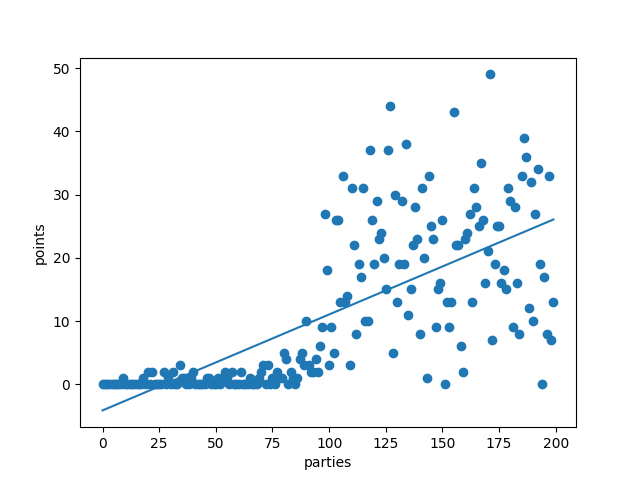
\includegraphics[width=\linewidth]{scatter_score_200_games.png}
	\caption{Nuage de points du pointage par rapport au nombre de parties jouées.}
	\label{fig:Snake}
\end{figure}

La première figure montre le pointage par rapport au nombre de parties jouées. On peut voir que le pointage lors de la période d’exploration reste bas. Ceci  s'explique par le fait que le serpent effectue des actions aléatoires et se rend rarement à la nourriture. On voit toutefois qu’il apprend correctement et obtient de bons scores avec une moyenne de 10.965 points par parties et un score maximal de 49 points. Une limitation du modèle est que l’état utilisé ne permet pas de représenter si le serpent s’enroule sur lui même. Cette situation arrive plus souvent lorsque le score devient haut et est une raison pourlaquelle le score semble stagner après un certain nombre de parties. La probabilité d’action aléatoire reste présente pendant tout l'entrainement, ce qui peut causer certaines anomalies, mais reste important pour éviter de tomber dans un état de boucle infinie.

\begin{figure}[ht]
	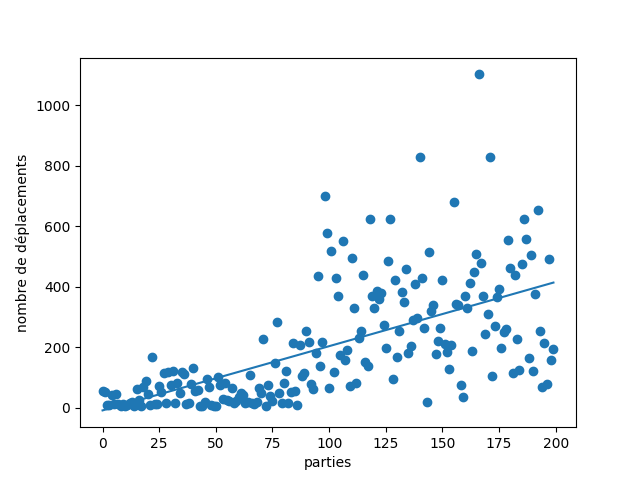
\includegraphics[width=\linewidth]{moves_per_game_200.png}
	\caption{Nuage de points du nombre de déplacements par rapport au nombre de parties jouées.}
	\label{fig:Snake}
\end{figure}

La deuxième figure présente le nombre d'actions par rapport au nombre de parties jouées. Cette figure nous permet de bien visualiser le fait que même si au début de l'entrainement le score est bas, l'agent progresse quand même en ce sens qu'il survit plus longtemps. C'est donc dire que l'agent apprend tout d'abord à survivre pour ensuite apprendre à faire des points.  

En observant l'agent jouer, il est évident que son comportement soit limité. L'agent peut seulement interpréter les dangers imminents et a tendance à s'entremêler sur lui même et perdre. Cette limitation cause un plateau que l'agent ne semble pas surpasser même avec un entrainement plus long.


Pour une meilleure vue d'ensemble, voici un lien vers une capture d’un entrainement pour visualiser le comportement du serpent ainsi qu'un lien vers le répertoire Git avec le code source de l'implémentation proposée.

Youtube:
\scriptsize\href{https://www.youtube.com/watch?v=HNeuuXA3Flg&feature=youtu.be}{https://www.youtube.com/watch?v=HNeuuXA3Fl\&feature=youtu.be}

\normalsize GitHub: 
\href{https://github.com/Adrimeov/snakeAI}{https://github.com/Adrimeov/snakeAI}


\section{Améliorations possibles}

Une difficulté observée était que le modèle semblait seulement apprendre à survivre. Nous avons expérimenté de différentes façons pour altérer ce comportement. Par exemple, nous avons modifié le système de récompenses afin de bonifier l’agent lorsque le serpent mange ou simplement ajouté une récompense positive lorsqu’il se déplace sans perdre. Le comportement ne semblait pas changer selon les récompenses. Le problème apparaissait à cause de l’entrainement qui est effectué avec la mémoire entre chaque époque. Lors des premières parties, le serpent réussissait rarement à manger donc sa mémoire était remplie d’états où les récompenses sont nulles ou négatives. Il apprenait donc seulement à se déplacer et éviter les dangers. La solution choisie était de sauvegarder un ensemble équilibré de mémoires qui représentent les différentes récompenses. Après avoir fait ce changement, le serpent vite compris à gérer les différentes solutions.

La solution proposée est très spécifique au jeu Snake et beaucoup de changements seraient nécessaires si nous voulions l’adapter pour un autre jeu. L’état donné à l’agent, soit la dimension de l’entrée du modèle, n’est valable que pour ce jeu et nous pouvons dire la même chose du vecteur d’action. Une solution possible pour rendre l’état générique serait d’utiliser l’image du jeu comme entrée. Cette technique permet de ne pas avoir à extraire manuellement un vecteur qui représente l’environnement du joueur. Sinon, il serait possible d’expérimenter avec des réseaux convolutifs ou d’autres techniques plus intéressantes qu’un simple réseau de neurones profond.

\section{Conclusion}

Nous avons commencé ce rapport en explorant brièvement l'historique concernant l'apprentissage par renforcement. Cette revue de la littérature nous a permis de nous faire une bonne idée des techniques utilisées. Afin de mettre en pratique ces nouvelles connaissances, nous avons décidé d'implémenter la méthode décrite dans le papier de Mnih et al. \cite{DBLP:journals/corr/MnihKSGAWR13} avec certaines modifications inspirées du blog de Comi \cite{comi_2020}. Nous avons donc expliqué les détails théoriques derrière cette implémentation. Par la suite, nous avons explicité concrètement comment nous avons pu reproduire les résultats des papiers desquels nous nous sommes inspirés. Nous avons montré les résultats que notre implémentation à pu produire. Nous avons montré que notre agent apprenait bien les détails du jeu de Snake. Finalement, nous avons proposé certaines améliorations (i.e intégrer un réseau à convolution avec la représentation en image du jeu) afin d'améliorer la performance de notre agent. 

\printbibliography
\end{document}

